\documentclass{report}

\usepackage{amsmath}
\usepackage{amssymb}
\usepackage{stmaryrd}
\usepackage{geometry}
\usepackage{tkz-tab}
\usepackage{tcolorbox}

\geometry{a4paper, left=20mm, right=20mm, top=20mm, bottom=20mm}

\begin{document}
\setcounter{chapter}{14}

\setcounter{section}{1}
\section{Exercice}
\begin{enumerate}
    \item Soit $k \geq 2 \in \mathbb{N}$. \\
    \begin{align*}
        \frac{1}{k^2} \leq \frac{1}{k-1} - \frac{1}{k} &\Leftrightarrow \frac{1}{k^2} \leq \frac{1}{k(k-1)} \\
        &\Leftrightarrow \frac{1}{k} \leq \frac{1}{k-1} \\
        &\Leftrightarrow k \geq k-1 \text{ ($x \mapsto \frac{1}{x}$ est décroissante)}
    \end{align*}

    \item On suppose que $S_n$ converge. Ainsi, pour $n \in \mathbb{N}$, on a d'une part : 
    \begin{align*}
        \frac{1}{k^2} \leq \frac{1}{k-1} - \frac{1}{k}
        &\Leftrightarrow S_n \leq 1 + \sum_{k=2}^{n} \left( \frac{1}{k-1} - \frac{1}{k} \right) \\
        &\Leftrightarrow S_n \leq 1 + 1 - \frac{1}{n} \text{ (télescopage)} \\
        &\Leftrightarrow \lim_{n \to +\infty} S_n \leq \lim_{n \to +\infty} 2 + \frac{1}{n} \text{ (Hypothèse)}\\
        &\Leftrightarrow \lim_{n \to +\infty} S_n \leq 2
    \end{align*}
    D'autre part, la suite est strictement croissante, donc d'après le théorème de la limite monotone, $(u_n)$ converge. 
\end{enumerate}

\setcounter{section}{5}
\section{Exercice}
\begin{enumerate}
    \item Soit $n \in \mathbb{N}$. Lorsque $a = 1$, on a la relation $u_{n+1} = u_n + b$. 
    Ainsi, $(u_n)$ est une suite arithmétique d'expression : 
    $$u_n = u_0 + nb$$

    \item \begin{enumerate}
        \item Pour $n \in \mathbb{N}$ : 
        \begin{align*}
            v_n &= u_n + \lambda \\
            \text{donc } v_{n+1} &= u_{n+1} + \lambda \\
            &= a u_{n} + b + \lambda
        \end{align*}
        On remarque que pour $\lambda = \frac{b}{a-1}$ avec $a \neq 1$, on a :
        \begin{align*}
            v_{n+1} &= a u_n + b + \frac{b}{a - 1} \\
            &= \frac{(a-1) (a) u_n + (a-1)b + b}{a - 1} \\
            &= a \times \frac{(a-1) u_n + b}{a-1} \\
            &= a \left( u_n + \frac{b}{a - 1} \right) \\
            &= a v_n
        \end{align*}
        Donc pour $\lambda = \frac{b}{a-1}$, $(v_n)$ est géométrique. 

        \item \begin{align*}
            v_n &= u_n + \frac{b}{a-1} \\
            \text{donc } u_n &= v_n - \frac{b}{a-1} \\
            &= \left( u_0 + \frac{b}{a-1} \right) \times a^n - \frac{b}{a-1} \\
            &= u_0 a^n + (a^n - 1) \frac{b}{a-1}
        \end{align*}
    \end{enumerate}
\end{enumerate}

\setcounter{section}{8}
\section{Exercice}
On s'intéresse aux suites extraites $(u_{e^{2\pi n}})$ et $(u_{e^{2\pi n + \pi}})$ : 
\begin{align*}
    (u_{e^{2\pi n}}) &= (\cos (2\pi n)) \\
    (u_{e^{2\pi n + \pi}}) &= (\cos (2\pi n + \pi))
\end{align*}
On a les limites : 
\begin{align*}
    u_{e^{2\pi n}} &\underset{n \to +\infty}{\longrightarrow} 1 \\
    u_{e^{2\pi n + \pi}} &\underset{n \to +\infty}{\longrightarrow}  -1
\end{align*}
Les deux suites extraites ne convergent pas vers la même limite, donc la suite $(u_n)$ n'a pas de limites. 

\section{Exercice}
\begin{enumerate}
    \setcounter{enumi}{2}
    \item Soit $x \in [0, 1]$. Soit $\epsilon > 0$. \\
    Par \textbf{densité} de $\mathbb{Q}$ dans $\mathbb{R}$, on choisi $q = \frac{a}{b} \in \mathbb{Q}$ tel qu $|x-q|<\frac{\epsilon}{2}$. \\
    D'après la question 2, comme $u_{n^2 b^2 + 2an} \underset{n \to +\infty}{\longrightarrow} \frac{a}{b} = q$, on choisit $n \in \mathbb{N}$ tel que : 
    $$|u_{n^2b^2+2an} - q| < \frac{\epsilon}{2} \text{ et } |u_n - x| < \epsilon$$
    Donc $\{u_n, n\in \mathbb{N} \}$ est dense dans $[0,1]$. \\
    D'après le critère séquentiel de la densité, tout réel de $[0,1]$ est donc une limite d'une suite extraite de $u$. 
\end{enumerate}

\setcounter{section}{11}
\section{Exercice}
\begin{enumerate}
    \item Soit $n \in \mathbb{N}^*$ et $u_n = (-1)^n + \frac{1}{n}$. \\
    Soit $k \in \mathbb{N}$. 
    \begin{align*}
        \begin{cases}
            1 \leq (-1)^{2k} + \frac{1}{2k} \leq \frac{3}{2} \\
            -1 \leq (-1)^{2k+1} + \frac{1}{2k+1} \leq 0
        \end{cases}
        \text{ donc } 
        -1 \leq (-1)^n + \frac{1}{n} \leq \frac{3}{2}
    \end{align*}
    $u_2 = \frac{3}{2}$, donc d'après la caractérisation séquentielle de la borne supérieure, $\sup \left\{ (-1)^n + \frac{1}{n} \right\} = \frac{3}{2}$. \\
    De plus, $u_{2n+1} \underset{n \to +\infty}{\longrightarrow} -1$, donc d'après la caractérisation séquentielle de la borne inférieure, $\inf \left\{ (-1)^n + \frac{1}{n} \right\} = -1$. 
\end{enumerate}
\begin{enumerate}
    \setcounter{enumi}{1}
    \item Soit $(p,q) \in \mathbb{Z}^2$ avec $p \neq q$ et $v_{p,q} = \frac{1}{p-q}$. \\
    Pour tout $(p,q) \in \mathbb{Z}^2$ avec $p \neq q$, on a : $p-q \in \mathbb{Z}^* = \mathbb{Z} \setminus {0}$ \\
    Si $p-q > 0$, alors $\frac{1}{p-q} > 0$ et $\frac{1}{p-q} \leq 1$ car $p-q \geq 1$ \\
    Si $p-q < 0$, alors $\frac{1}{p-q} < 0$ et $\frac{1}{p-q} \geq -1$ car $p-q \leq -1$ \\
    Donc $-1 \leq \frac{1}{p-q} \leq 1$ \\
    De plus, on peut prendre $p=0$ et $q=1$ pour obtenir $v_{0,1} = -1$, et $p=1$ et $q=0$ pour obtenir $v_{1,0} = 1$ \\
    D'après la caractérisation séquentielle de la borne supérieure et de la borne inférieure : \\
    $\sup \left\{ \frac{1}{p-q} \right\}{(p,q)\in\mathbb{Z}^2, p\neq q} = 1$ et $\inf \left\{ \frac{1}{p-q} \right\}{(p,q)\in\mathbb{Z}^2, p\neq q} = -1$
    
    \item Soit $k \in \mathbb{N}^*$ et $w_k = \frac{(-1)^k k}{k+1}$. \\
    Pour tout $k \in \mathbb{N}^*$ : \\
    Si $k$ est pair, alors $w_k = \frac{k}{k+1} > 0$ et $w_k < 1$ \\
    Si $k$ est impair, alors $w_k = -\frac{k}{k+1} < 0$ et $w_k > -1$ \\
    Donc $-1 < \frac{(-1)^k k}{k+1} < 1$ \\
    De plus, pour $k$ pair, $w_k = \frac{k}{k+1} \underset{k \to +\infty}{\longrightarrow} 1$ \\
    Et pour $k$ impair, $w_k = -\frac{k}{k+1} \underset{k \to +\infty}{\longrightarrow} -1$ \\
    D'après la caractérisation séquentielle de la borne supérieure et de la borne inférieure : \\
    $\sup \left\{ \frac{(-1)^k k}{k+1} \right\}_{k\in\mathbb{N}^*} = 1$ et $\inf \left\{ \frac{(-1)^k k}{k+1} \right\}_{k\in\mathbb{N}^*} = -1$
\end{enumerate}

\section{Exercice}
D'une part, on a : 
\begin{align*}
    u_{n+1} - u_n &= \sum_{k=n+2}^{2n+2} \frac{1}{k} - \sum_{k=n+1}^{2n} \frac{1}{k} \\
    &= \frac{1}{2n+1} + \frac{1}{2n+2} - \frac{1}{n+1} \\
    &= \frac{1}{2n+1} - \frac{1}{2n+2} \\
    &\geq 0
\end{align*}
Donc $(u_n)$ est bien croissante. \\
D'autre part, on a : 
\begin{align*}
    v_{n+1} - v_n &= \sum_{k=n+2}^{2n+2} \frac{1}{k} - \sum_{k=n}^{2n} \frac{1}{k} \\
    &= \frac{1}{2n+1} + \frac{1}{2n+2} - \frac{1}{n} \\
    &= \frac{-3n+3}{(2n+1)(2n+2)n}
    \leq 0 \text{ (car $n \in \mathbb{N}^*$)}
\end{align*}
Donc $(v_n)$ est bien décroissante. \\ \\
En outre : 
\begin{align*}
    u_n - v_n &= \sum_{k=n+1}^{2n} \frac{1}{k} - \sum_{k=n}^{2n} \frac{1}{k} \\
    &= -\frac{1}{n} \\
    &\underset{n \to +\infty}{\longrightarrow} 0
\end{align*}
Donc $u$ et $v$ sont bien des suites adjacentes. 

\setcounter{section}{16}
\section{Exercice}
\begin{enumerate}
\item Montrons que pour tout $x \geq 3$, la fonction $x \mapsto \frac{2x^2 - 3}{x+2}$ est minorée par $3$ : \\
On note $f$ la fonction $x \mapsto \frac{2x^2 - 3}{x+2}$. \\
\begin{align*}
    f'(x) &= \frac{2x^2+8x+3}{(x+2)^2} \\
    f'(x) = 0 &\Leftrightarrow 2x^2 + 8x + 3 = 0 \\
    &\Leftrightarrow x = 2 \pm \sqrt{\frac{5}{2}}
\end{align*}
On a donc le tableau de variations suivant : \\ \\
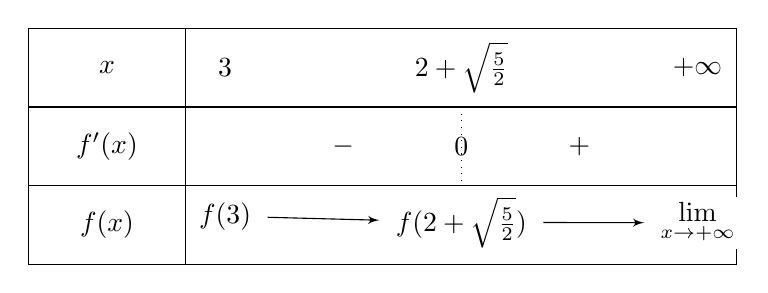
\begin{tikzpicture}
    \tkzTabInit{$x$ / 1, $f'(x)$ / 1, $f(x)$ / 1}{$3$, $2 + \sqrt{\frac{5}{2}}$, $+\infty$}
    \tkzTabLine{,-,z,+,}
    \tkzTabVar{+/ $f(3)$, -/ $f(2+\sqrt{\frac{5}{2}})$, +/ $\lim\limits_{x \to +\infty} $}
\end{tikzpicture} \\

\noindent Ainsi, $[3, +\infty[$ est stable par la fonction $f$. 

\item \begin{enumerate}
    \item a
\end{enumerate}
\end{enumerate}

\end{document}